%

\index{aksjomaty!Hilberta|(}%

\section{Aksjomaty Hilberta}

W aksjomatyce Hilberta (płaskiej geometrii euklidesowej) pojęciami pierwotnymi są punkt, prosta, płaszczyzna, relacja incydencji (leżeć na, zawierać się w), relacja uporządkowania (leżenia między) oraz relacja przystawania.
Wszystkie aksjomaty w jednym miejscu wymienia Eves \cite[s. 380-382]{eves1_1972}.

Punkty i proste będziemy oznaczać wielkimi i małymi literami alfabetu łacińskiego.

%

\index{aksjomaty!incydencji|(}%

\subsection{Aksjomaty incydencji}
\begin{axiom}[incydencji, I1]
    Dla każdej pary punktów $A$ oraz $B$ istnieje dokładnie jedna prosta $l$, która przechodzi przez te punkty.
\end{axiom}

Zdania ,,prosta $l$ przechodzi przez punkt $A$'' oraz ,,punkt $A$ leży na prostej $l$'' mają dokładnie to samo znaczenie i będziemy je stosować zamiennie.

\begin{axiom}[incydencji, I2]
    Na każdej prostej leżą co najmniej dwa punkty.
\end{axiom}

\begin{axiom}[incydencji, I3]
    Istnieją co najmniej trzy punkty, które nie są współliniowe.
\end{axiom}

,,Być współliniowym'' to synonim leżenia na jednej prostej.
\index{współliniowy}%
Analogicznie mówimy, że wiele prostych, które przechodzą przez jeden punkt, jest współpękowych.

\begin{proposition}
    Dwie różne proste mogą mieć co najwyżej jeden punkt wspólny.
\end{proposition}

\begin{definition}
    Dwie różne proste, które nie są współpękowe (nie mają punktów wspólnych), nazywamy równoległymi.
    Każda prosta jest też równoległa do siebie.
\end{definition}
\index{prosta!równoległa}%

Trzeba uważać, bo dla niektórych dwie proste równoległe są współpękowe, bo przechodzą przez punkt w nieskończoności, jak zwykło się mawiać w geometrii rzutowej (niektórzy bowiem rozróżniają współpękowość właściwą i niewłaściwą).
Na dwóch prostych, które nie są równoległe, leży dokładnie jeden punkt.
Mówimy, że proste się przecinają, a wspomniany punkt jest ich punktem przecięcia.
Symbolicznie: $k \parallel l$ albo $k \nparallel l$ (wtedy $k \cdot l$ to jedyny punkt leżący na obydwu prostych).

Hartshorne \cite[s. 38]{hartshorne2000} przywoła:

\begin{axiom}[Playfaira, P]
    Dla każdej prostej $l$ oraz punktu $A$, istnieje co najwyżej jedna prosta, która przechodzi przez $A$ i jest równoległa do $l$.
\end{axiom}
\index{aksjomat!Playfaira}%
% TODO: https://en.wikipedia.org/wiki/Playfair%27s_axiom

John Playfair opublikuje ten aksjomat w 1795 roku, chociaż już wtedy stwierdzi, że inni używali go przed nim (np. William Ludlam).
\index[persons]{Playfair, John}%
\index[persons]{Ludlam, William}%
Aksjomat Playfaira jest równoważny z (piątym) postulatem Euklidesa i dlatego wiele osób spróbuje wyprowadzić go z czterech wcześniejszych postulatów.
Za każdym razem okaże się, że w ,,dowodzie'' użyte jest zdanie będące równoważnikiem piątego postulatu, na przykład:
\begin{itemize}
    \item suma kątów wewnętrznych pewnego trójkąta jest kątem półpełnym,\index{suma kątów}%
    \item suma kątów wewnętrznych każdego trójkąta jest kątem półpełnym,\index{suma kątów}%
    \item suma kątów wewnętrznych każdego trójkąta jest taka sama,\index{suma kątów}%
    \item istnieją dwa trójkąty, które są do siebie podobne, ale nie przystające,\index{podobieństwo}\index{przystawanie}%
    \item na każdym trójkącie można opisać okrąg,\index{okrąg!opisany}%
    \item istnieje para prostych, które są w stałej odległości od siebie,
    \item dwie proste, które są równoległe do danej prostej, są też równoległe do siebie,\index{prosta!równoległa}%
    \item twierdzenie Pitagorasa lub jego uogólnienie, twierdzenie cosinusów,\index{twierdzenie!Pitagorasa}\index{twierdzenie!cosinusów}%
    \item aksjomat Wallisa: nie ma górnego ograniczenia na pole trójkąta,\index{aksjomat!Wallisa}%
    \item aksjomat Proklosa: jeśli prosta przecina jedną z dwóch równoległych prostych, to przecina także tę drugą,\index{aksjomat!Proklosa}%
    \item kąty przy górnej podstawie czworokąta Saccheriego (czworokąta $ABCD$ o dwóch kątach prostych przy dolnej podstawie $AB$, w którym boki $AD$ i $BC$ mają równe długości) są proste,\index{czworokąt!Saccheriego}%
    \item jeśli trzy kąty wewnętrzne czworokąta są proste, to czwarty kąt także jest prosty (czworokąt Lamberta jest prostokątem).\index{czworokąt!Lamberta}%
% https://en.wikipedia.org/wiki/Saccheri_quadrilateral
\end{itemize}

% TODO: https://en.wikipedia.org/wiki/Parallel_postulate

https://www.deltami.edu.pl/2012/05/dowody-v-postulatu-euklidesa/

\begin{example}
    Rozważmy geometrię, gdzie płaszczyzna składa się z pięciu punktów $A$, $B$, $C$, $D$, $E$ i leży na niej dziesięć różnych prostych, każda z nich przechodząca przez dokładnie dwa różne punkty.
    Wtedy proste $AB$ i $AC$ mają punkt wspólny $A$, chociaż obydwie są równoległe do prostej $DE$.
    Aksjomat Playfaira nie jest spełniony. \index{aksjomat!Playfaira}
\end{example}

\begin{proposition}
    Aksjomaty incydencji I1, I2, I3 oraz aksjomat P (Playfaira) są od siebie niezależne. \index{aksjomat!Playfaira}
\end{proposition}

Hartshorne \cite[s. 69-70]{hartshorne2000} konstruuje modele geometrii, w których spełnione są dowolne trzy, ale nie czwarty z nich.

\begin{proposition}
    Płaszczyzna rzutowa to taki zbiór punktów oraz prostych (podzbiorów zbioru punktów), że: \index{płaszczyzna!rzutowa}
    \begin{itemize}
        \item przez dwa różne punkty przechodzi dokładnie jedna prosta,
        \item każde dwie proste mają punkt wspólny,
        \item każda prosta ma co najmniej trzy punkty i
        \item nie wszystkie punkty są współliniowe.
    \end{itemize}
    (Każdy z wymienionych aksjomatów jest niezależny od pozostałych, ze wszystkich razem wynikają aksjomaty incydencji).
    Każda płaszczyzna rzutowa ma co najmniej 7 punktów, dokładnie jedna płaszczyzna rzutowa ma dokładnie 7 punktów.
    Jeśli istnieje prosta, która ma $n+1$ punktów, to płaszczyzna ma $n^2 + n + 1$ punktów.
\end{proposition} % Hartshorne 71

https://www.deltami.edu.pl/2013/05/dziewiec-twarzy-plaszczyzny-rzutowej/ % TODO

\begin{example}[płaszczyzna Fana]
    Zbiór złożony z siedmiu elementów (,,punktów''), w którym wyróżniono rodzinę siedmiu podzbiorów (,,prostych'') spełniający następujące warunki: \index{płaszczyzna!Fana}
    \begin{itemize}
        \item każde dwie różne proste mają dokładnie jeden punkt wspólny,
        \item każde dwa różne punkty należą do dokładnie jednej prostej
    \end{itemize}
    nazywamy płaszczyzną Fana.
    Jest przykładem płaszczyzny rzutowej, która nie spełnia aksjomatu Fana (że trzy punkty przekątne czworoboku zupełnego nie są współliniowe). \index{aksjomat Fana}
    \begin{figure}[H]
        \centering
        \begin{tikzpicture}[
        mydot/.style={
        draw,
        circle,
        fill=black,
        inner sep=1.5pt}
        ]
        \draw
        (0,0) coordinate (A) --
        (4cm,0) coordinate (B) --
        ($ (A)!.5!(B) ! {sin(60)*2} ! 90:(B) $) coordinate (C) -- cycle;
        \coordinate (O) at
        (barycentric cs:A=1,B=1,C=1);
        \draw (O) circle [radius=4cm*1.717/6];
        \draw (C) -- ($ (A)!.5!(B) $) coordinate (LC); 
        \draw (A) -- ($ (B)!.5!(C) $) coordinate (LA); 
        \draw (B) -- ($ (C)!.5!(A) $) coordinate (LB); 
        \foreach \Nodo in {A,B,C,O,LC,LA,LB}
        \node[mydot] at (\Nodo) {};    
    \end{tikzpicture}%
    \caption{Płaszczyzna Fana z 1892 roku}
\end{figure}
\end{example}

Jest po jednej płaszczyźnie rzutowej dla $n = 3, 4, 5, 6, 8$ punktów na każdej prostej; żadnej dla $n = 7$, co najmniej jedna dla $n = 9$ i co najmniej cztery dla $n = 10$.
O płaszczyźnie Fana napisze Eves \cite[s. 366]{eves1_1972}.

W momencie pisania tego tekstu nie jesteśmy jeszcze zainteresowani geometrią rzutową, więc przytoczymy tylko wymagania wobec studenta, który ukończył kurs ,,Geometria III'' na uniwersytecie w Warszawie.
Audin \cite[s. 143-182]{audin_2003}.
Delta: 2024/lipiec.

Zna pojęcie płaszczyzny rzutowej rzeczywistej (równoważne sformułowania), dwustosunku, definicję przekształceń rzutowych łańcuchów, stożkowych, pęków stycznych do stożkowych.
\index{dwustosunek}%
\index{pęk}%
\index{stożkowa}%
Zna i~potrafi stosować twierdzenia Steinera i Braikenridge'a-Maclaurina.
\index{twierdzenie!Steinera}%
\index{twierdzenie!Braikendridge'a-Maclaurina}%
Wie w jaki sposób określa się rzutowo ogniska i kierownice stożkowych.
\index{ognisko}%
\index{kierownica}%

\begin{proposition}
    Płaszczyzna afiniczna to taki zbiór punktów i prostych, które spełniają: \index{płaszczyzna!afiniczna}
    \begin{itemize}
        \item aksjomaty incydencji oraz
        \item mocniejszą wersję aksjomatu Playfaira: dla każdej prostej $l$ i punktu $A$, dokładnie jedna prosta przechodzi przez punkt $A$ i jest równoległa do $l$.
    \end{itemize}
    Każda prosta na płaszczyźnie afinicznej ma tyle samo punktów.
    Jeśli pewna prosta ma $n$ punktów, to płaszczyzna ma dokładnie $n^2$ punktów.
    Istnieją płaszczyzny afiniczne o $4$, $9$, $16$ i $25$ punktach, ale nie istnieje taka, która miałaby $36$ punktów.
\end{proposition} % Hartshorne 71, 72

Podręcznik Audina \cite[s. 7]{audin_2003} zaczyna się od definicji przestrzeni afinicznej.
Coxeter \cite[s. 209]{coxeter_1967} wspomni, że według Blaschkego słowo ,,afiniczny'' utworzył Euler.

My nie poświęcimy powinowactwu (bo tak tłumaczy się na polski słowo \emph{affinity}) za dużo miejsca; znajdzie się w niektórych numerach czasopisma Delta: $\Delta_{24}^6$.

\index{aksjomaty!incydencji|)}%

%
%

\index{aksjomaty!leżenia pomiędzy|(}%

\subsection{Aksjomaty leżenia pomiędzy}
O relacji między aksjomatami B1-B4 i uporządkowaniem ciała, nad którym pracujemy, rozwodzi się Hartshorne \cite[s. 135-140]{hartshorne2000}

\begin{axiom}[leżenia pomiędzy, B1]
    Jeśli punkt $B$ leży między punktami $A$ i $C$, to punkty $A$, $B$, $C$ są różnymi punktami tej samej prostej oraz punkt $B$ leży także między punktami $C$ i $A$.
\end{axiom}

\begin{axiom}[leżenia pomiędzy, B2]
    Dla każdej pary punktów $A$ i $B$ istnieje punkt $C$ taki, że punkt $B$ leży między punktami $A$ i $C$.
\end{axiom}

\begin{axiom}[leżenia pomiędzy, B3]
    Spośród trzech punktów leżących na prostej, dokładnie jeden leży pomiędzy pozostałymi dwoma.
\end{axiom}

\begin{axiom}[leżenia pomiędzy, B4]
    Niech $A$, $B$ i $C$ będą trzema niewspółliniowymi punktami, zaś $l$ prostą, która nie przechodzi przez żaden z nich.
    Jeśli prosta $l$ przechodzi przez punkt między punktami $A$ i $B$, to przechodzi też przez punkt między punktami $A$ i $C$ albo $B$ i $C$, ale nie przez obydwa.
\end{axiom}

Powyższy aksjomat nazywany jest też aksjomatem Pascha, ponieważ Moritz Pasch \cite{pasch_1882} przyłapał dopiero w 1882 roku geometrów całego świata na tym, że korzystali z takiej przesłanki.
\index{aksjomat!Pascha}%
\index[persons]{Pasch, Moritz}%
Aksjomatu Pascha (B4) nie wolno mylić z aksjomatem Veblena-Younga geometrii rzutowej\footnote{Jeśli prosta przecina dwa boki trójkąta, to przecina także jego trzeci bok. \index{aksjomat!Veblena-Younga}}!
% PRZEJRZANO: https://en.wikipedia.org/wiki/Pasch%27s_axiom

\begin{proposition}
    Z aksojmatów I1 do I3, B1 do B4 wynika, że każda prosta ma nieskończenie wiele punktów.
\end{proposition}

\begin{definition}[odcinek]
    Niech $A$, $B$ będą punktami.
    Zbiór złożony z punktów $A$, $B$ oraz punktów, które leżą między nimi, nazywamy odcinkiem i oznaczamy:
\index{odcinek}%
    \begin{equation}
        \overline{AB}.
    \end{equation}
\end{definition}

Jeżeli nie prowadzi to do nieporozumień, kreskę pomijamy.

\begin{definition}[trójkąt]
    Niech $A$, $B$, $C$ będą punktami.
    Sumę odcinków $AB$, $BC$, $AC$ nazywamy trójkątem, wspomniane odcinki -- jego bokami, zaś punkty $A$, $B$ i $C$ -- wierzchołkami.
\index{trójkąt}%
\end{definition} % Hartshorne 74

Trójkąty zazwyczaj oznaczamy tak: $\triangle ABC$ i nie odróżniamy go od trójkąta z wnętrzem.
Mamy podział na trójkąty ostrokątne (z trzema kątami ostrymi), prostokątne (z jednym kątem prostym), rozwartokątne (z jednym kątem większym niż prosty), ale też na: równoboczne (z trzema bokami, które są przystające), równoramienne (z dwoma przystającymi bokami zwanymi ramionami, wtedy trzeci bok nazywa się podstawą) albo różnoboczne, z angielskiego \emph{scalene}.

\begin{proposition}
    Niech $l$ będzie prostą.
    Wtedy zbiór punktów, które nie leżą na prostej $l$ można rozbić na dwa niepuste zbiory $S_1$, $S_2$ takie, że: dwa punkty, które nie leżą na prostej $l$, należą do tego samego zbioru ($S_1$ lub $S_2$) wtedy i~tylko wtedy, gdy odcinek $AB$ nie przecina prostej $l$.
\end{proposition} % Hartshorne 74

Zbiory $S_1$, $S_2$ nazywamy stronami prostej $l$.
\index{prosta!dwie strony prostej}%
Podobnie punkt wyznacza na prostej dwa zbiory, które leżą po różnych stronach tego punktu.

\begin{definition}[półprosta]
    Niech $A$, $B$ będą punktami.
    Zbiór złożony z punktów $A$, $B$ oraz punktów, które leżą po tej samej stronie punktu $A$ na prostej $AB$ co punkt $B$, nazywamy półprostą i oznaczamy:
\index{półprosta}%
    \begin{equation}
        \overrightarrow{AB}.
    \end{equation}
\end{definition} % Hartshorne 77

Ponownie, strzałkę psującą interlinię często pomijamy.

\begin{definition}[kąt]
    Sumę dwóch półprostych $AB$, $AC$, które nie leżą na jednej prostej, nazywamy kątem, zaś punkt $A$ wierzchołkiem tego kąta.
    Wnętrze kąta $\angle BACS$ składa się z tych punktów $D$ takich, że $D$ i $C$ leżą po tej samej stronie prostej $AB$ oraz $D$ i $B$ leżą po tej samej stronie prostej $AC$. 
    \index{kąt}%
\end{definition} % Hartshorne 77

W myśl tej definicji, nie ma kąta zerowego, wklęsłego ani półpełnego.
\index{kąt!zerowy}%
\index{kąt!półpełny}%
\index{kąt!wklęsły}%
Wnętrze trójkąta $ABC$ to część wspólna wnętrz kątów $\angle ABC$, $\angle BCA$, $\angle CAB$; jest wypukłe (jeśli dwa punkty końce odcinka należą do wnętrza, to również każdy inny punkt tego odcinka znajduje się tam) i niepuste.

\index{aksjomaty!leżenia pomiędzy|)}%

%
\index{aksjomaty!przystawania|(}%
%

\subsection{Aksjomaty przystawania odcinków}
Listę aksjomatów rozszerzymy o trzy, które opisują niezdefiniowane pojęcie przystawania odcinków: relacji między odcinkami, którą oznaczamy przez $\cong$.

\begin{axiom}[przystawania, C1]
    Niech $A$ i $B$ będą punktami, zaś $l$ prostą przechodzącą przez punkt $C$.
    Wtedy po każdej stronie punktu $C$ istnieje punkt $D$ taki, że odcinki $AB \cong CD$ są przystające.
\end{axiom}

Ten aksjomat odpowiada konstrukcji (I.3) Euklidesa i pozwala przenosić odcinki.
\index{odcinek!przenoszenie}%

\begin{axiom}[przystawania, C2]
    Jeśli $AB \cong CD$ oraz $AB \cong EF$, to $CD \cong EF$.
    Każdy odcinek jest przystający do siebie.
\end{axiom}

To było pierwsze pojęcie pierwotne dla Euklidesa.

\begin{axiom}[przystawania, C3]
    Niech $A$, $B$, $C$, $D$, $E$, $F$ będą takimi punktami, że $B$ leży między $A$ i $C$, zaś $E$ leży między $D$ i $F$.
    Jeśli $AB \cong DE$ i $BC \cong EF$, to $AC \cong DF$.
\end{axiom}

Ten aksjomat pozwala nam dodawać odcinki i znowu zastępuje pojęcie pierwotne Euklidesa.
Dodawanie jest łączne i przemienne.

\begin{proposition}[odejmowanie odcinków]
    Niech $A$, $B$, $C$, $D$, $E$, $F$ będą takimi punktami, że $B$ leży między $A$ i $C$, zaś $E$ i $F$ leżą na półprostej zaczynającej się w $D$.
    Jeśli $AB \cong DE$ i $AC \cong DF$, to punkt $E$ leży między $D$ i $F$, co więcej $BC \cong EF$.
\end{proposition}

Odcinek $BC$ traktujemy jako różnicę między $AC$ i $AB$.
Dla Euklidesa to było pojęcie pierwotne (że całość jest większa od części).

\begin{definition}
    Niech $AB$ i $CD$ będą odcinkami.
    Jeśli istnieje punkt $E$ między $C$ i $D$ taki, że $AB \cong CE$, to powiemy, że odcinek $AB$ jest krótszy niż odcinek $CD$ (zaś odcinek $CD$ jest dłuższy niż odcinek $AB$).
\end{definition} % Hartshorne 85

Relacja bycia krótszym jest zgodna z przystawaniem i zadaje zupełny porządek na klasach równoważności.
Dodawanie odcinków zachowuje nierówności między nimi.

\begin{definition}[okrąg]
    Niech $O$, $A$ będą dwoma różnymi punktami.
    Zbiór punktów $B$ takich, że $OA \cong OB$ nazywamy okręgiem o środku $O$ oraz promieniu $OA$; okręgi często oznacza się literą $\Gamma$.
    \index{okrąg}
\end{definition} % Hartshorne 89

\begin{proposition}
    Każda prosta, która przechodzi przez środek, przecina okrąg w dwóch punktach.
    Okrąg składa się z nieskończenie wielu punktów.
\end{proposition}

(Nie jest jasne, ile środków może mieć okrąg, ale Hartshorne \cite[s. 89]{hartshorne2000} obiecuje pokazać póżniej, że tylko jeden.
\index{okrąg!środek okręgu}%
Później ma miejsce na stronie 104).

\begin{definition}[styczna]
    Niech $\Gamma$ będzie okręgiem, zaś $l$ prostą, która przecina $\Gamma$ w dokładnie jednym punkcie $A$.
    Mówimy, że $l$ jest styczną do okręgu $\Gamma$ w punkcie $A$.
    \index{styczność}
\end{definition}

Podobnie mówimy, że dwa okręgi są styczne, jeśli mają jeden punkt wspólny.
Neugebauer \cite[s. 20]{neugebauer_2018} podaje w formie ćwiczenia, że prosta i okrąg mają zawsze mniej niż trzy punkty wspólne.

%
%

\subsection{Aksjomaty przystawania kątów}
Dokładnie jak dla odcinków, wprowadzamy niezdefiniowaną relację przystawania kątów, oznaczaną znowu przez $\cong$, ponieważ nie prowadzi to do nieporozumień.

\begin{axiom}[przystawania, C4]
    Dla każdego kąta $\angle BAC$ i każdej $DF$ półprostej istnieje dokładnie jedna półprosta $DE$ po ustalonej stronie prostej $DF$ taka, że $\angle BAC \cong \angle EDF$.
\end{axiom}

Możemy traktować ten aksjomat jako odpowiednik cyrkla: pozwala przenosić kąty tak, jak Euklides (I.23).
\index{cyrkiel}

\begin{axiom}[przystawania, C5]
    Niech $\alpha, \beta, \gamma$ będą kątami.
    Jeśli $\alpha \cong \beta$ oraz $\alpha \cong \gamma$, to $\beta \cong \gamma$.
    Każdy kąt przystaje do siebie: $\alpha \cong \alpha$.
\end{axiom}

Mamy wreszcie cechę przystawania bok-kąt-bok, z której można wyprowadzić dodawanie kątów:
\index{cecha przystawania!bok-kąt-bok}%

\todofoot{kąt-bok-kąt: Neugebauer s. 8, bbb: Neuge s. 11}

\todofoot{Hartshorne s. 99: cechy przystawania!}
% bok bok bok / bok kąt bok / bok kąt kąt / kąt kąt kąt

\begin{axiom}[przystawania, C6]
    Niech $ABC$ i $DEF$ będą dwoma trójkątami takimi, że $AB \cong DE$, $AC \cong DF$ i $\angle BAC \cong \angle EDF$.
    Wtedy pozostałe boki i kąty są przystające, a razem z nimi całe trójkąty: $BC \cong EF$, $\angle ABC \cong \angle DEF$ i $\angle ACB \cong \angle DFE$.
\end{axiom}

Euklides udawał, że dowodzi aksjomatu C6 metodą ,,nakładania'' figur, ale Hilbert znalazł model będący świadkiem, że nie wynika on z poprzednich aksjomatów; patrz \cite[paragraf 11]{hilbert_1988}, jak wiemy od Greenberga \cite[s. 200]{greenberg_2010}.
(W obronie Euklidesa należy dodać, że metoda nakładania pojawia się dwa razy: w (I.4) oraz (I.8); gdyby była słuszna, postulat 4, że wszystkie kąty proste są równe, nie byłby potrzebny!).
\index{kąt!prosty}%
Patrz też do Hartshorne'a \cite[s. 148-158]{hartshorne2000}.

Jeżeli chodzi o dodawanie kątów, musimy być ostrożni.
Suma dwóch kątów może okazać się prostą (lub ,,dwoma kątami prostymi'' jak pisze Euklides) albo mieć miarę większą niż $\pi$, wtedy składniki sumy nie znajdują się we wnętrzu otrzymanego kąta.
Kąty można także odejmować.

\begin{definition}[kąt przyległy]
    Niech $\angle BAC$ będzie kątem, zaś $D$ punktem na prostej $AC$ po przeciwnej stronie $A$ niż $C$.
    Wtedy kąty $\angle BAC$ i $\angle BAD$ nazywamy przyległymi. % supplementary.
    \index{kąt!przyległy}
\end{definition}

Warto teraz spojrzeć na (I.13) Euklidesa.
(Są jeszcze kąty naprzemianległe i odpowiadające...)

\begin{figure}[H] \centering
\begin{comment}
\begin{tikzpicture}[scale=.6]
    \tkzDefPoint(-4, -2){A}
    \tkzDefPoint(4, 2){B}
    \tkzDefPoint(4, -2){C}
    \tkzDefPoint(-4, 2){D}
    \tkzDefPoint(0, 0){Zero}
    \tkzDefPoint(0, 0.7){X1}
    \tkzDefPoint(-1.7, 0){X2}
    \tkzDefPoint(1.7, 0){X3}
    \tkzMarkAngle[arc=l,size=1.2,mark=||](D,Zero,A)
    \tkzMarkAngle[arc=l,size=1.2,mark=||](C,Zero,B)
    \tkzMarkAngle[arc=ll,size=1.2](B,Zero,D)

    \tkzDrawSegments[line width=0.3mm](A,B)
    \tkzDrawSegments[line width=0.3mm](C,D)
    \tkzLabelPoint[anchor=center](X1){$\beta$}
    \tkzLabelPoint[anchor=center](X2){$\alpha$}
    \tkzLabelPoint[anchor=center](X3){$\gamma$}
\end{tikzpicture}
\end{comment}
    \caption{kąty przyległe ($\alpha$ i $\beta$) oraz wierzchołkowe ($\alpha$ i $\gamma$)}
\end{figure}

\begin{proposition}
\index{kąt!wierzchołkowy}%
    Kąty wierzchołkowe (para kątów przy dwóch przecinających się prostych, które nie są przyległe) są przystające.
\end{proposition}

Piszą o tym Bogdańska, Neugebauer \cite[s. 6]{neugebauer_2018}

% odpowiadające i naprzemianległe.
\todofoot{Pompe s. 5: dwie proste przecięte trzecią wyznaczają kąty tej samej miary <=> proste są równoległe (naprzemianległe). Pompe s. 5: suma kątów trójkąta to 180\index{suma kątów}}
% https://en.wikipedia.org/wiki/Saccheri-Legendre_theorem

Istnieje odpowiednik relacji między odcinkami ,,bycia mniejszym'' dla kątów:

\begin{definition}
    Niech $\angle BAC$ i $\angle EDF$ będą kątami.
    Jeśli istnieje półprosta $DG$ wewnątrz kąta $EDF$ taka, że $\angle BAC \cong \angle GDF$, to powiemy, że kąt $\angle BAC$ jest mniejszy niż kąt $\angle EDF$ (a ten drugi jest większy niż pierwszy).
\end{definition}

\begin{definition}
    Kąt, który przystaje do kąta przyległego, nazywamy prostym.
    Dwie proste, które przecinają się i wyznaczają tam cztery kąty proste, będziemy nazywać prostopadłymi.
\end{definition}

Nie jest ważne, który kąt przyległy wybierzemy, ponieważ kąty wierzchołkowe są przystające.

%
\index{aksjomaty!przystawania|)}%

\subsection{Płaszczyzna Hilberta}

Przedstawione do tej pory aksjomaty są niezbędnym minimum do uprawiania geometrii.

\begin{definition}
    Zbiór punktów i prostych, razem z relacjami leżenia pomiędzy, przystawania odcinków i kątów, które spełniają aksjomaty I1 do I3, B1 do B4, C1 do C6, nazywamy płaszczyzną Hilberta.
    \index{płaszczyzna!Hilberta}
\end{definition}

W szczególności, nie zakładamy aksjomatu równoległości (P).
\index{aksjomat!Playfaire'a}
Wszystkie twierdzenia Euklidesa od I.1 do I.28 (bez I.1, I.22) można udowodnić na dowolnej płaszczyźnie Hilberta.
Do dwóch wyjątków potrzebujemy dodatkowego aksjomatu \ref{axiom_e}.
\index{aksjomat!o części wspólnej dwóch okręgów}%

Potrzebujemy dodatkowego aksjomatu, by okręgi, od których oczekujemy, że się przetną, naprawdę się przecięły.
Wspomni o tym Coxeter \cite[s. 21]{coxeter_1967}.

\begin{axiom}[o części wspólnej dwóch okręgów, E]
    \label{axiom_e}
    Niech $\Gamma_1$, $\Gamma_2$ będą dwoma okręgami takimi, że każdy zawiera pewien punkt leżący wewnątrz drugiego.
    Wtedy istnieje punkt leżący na obydwu okręgach równocześnie.
    \index{aksjomat!o części wspólnej dwóch okręgów}%
\end{axiom}

Płaszczyznę Pitagorasa, która spełnia ten aksjomat, nazywamy płaszczyzną Euklidesa.
\index{płaszczyzna!Pitagorasa}

\begin{proposition}[o części wspólnej prostej i okręgu, LCI]
    Na płaszczyźnie Hilberta spełniającej aksjomat E, jeśli prosta $l$ zawiera punkt leżący wewnątrz okręgu $\Gamma$, to przecina ten okrąg.
    \index{aksjomat!o części wspólnej prostej i okręgu}
\end{proposition}

Dopiero teraz jesteśmy w stanie uratować twierdzenia (I.1), (I.22), (III.I), (III.17) z Elementów Euklidesa, do tego wszystkie dalsze wyniki aż do III.19 (ponieważ III.20 i dalej wymagany jest aksjomat Playfaira).
% [23, Exercise 16.11] gives an example of I.22 failure.
\index{aksjomat!Playfaire'a}

\todofoot{chord cięciwa, saggita, sieczna}

(Reszta tekstu tej sekcji na podstawie artykułu Greenberga \cite[s. 201]{greenberg_2010}).
Greenberg sugeruje nazywać płaszczyznę Hilberta, która spełnia aksjomat P, płaszczyzną Pitagorasa.
\index{płaszczyzna!Pitagorasa}%
\index{płaszczyzna!Hilberta}%

\begin{proposition}
    Każda płaszczyzna Pitagorasa jest izomorficzna z kwadratem $F^2$ pewnego uporządkowanego ciała $F$ takiego, że z $x, y \in F$ wynika $\sqrt{x^2 + y^2} \in F$.
\end{proposition}

\begin{proposition}
    Niech $F^2$ będzie płaszczyzną Pitagorasa.
    Następujące warunki są równoważne:
    \begin{itemize}
        \item z każdych trzech odcinków spełniających nierówność trójkąta można zbudować trójkąt; 
        \item aksjomat E jest spełniony na płaszczyźnie $F^2$.
    \end{itemize}
\end{proposition}

Aksjomat E pociąga za sobą prawdziwość aksjomatu LCI.
Patrz też do Hartshorne'a \cite[s. 144]{hartshorne2000}.

\begin{proposition}
    Niech $F^2$ będzie płaszczyzną Pitagorasa.
    Następujące warunki są równoważne:
    \begin{itemize}
        \item ciało $F$ jest euklidesowskie (każdy dodatni element $x \in F$ ma pierwiastek kwadratowy $\sqrt{x}$);
        \item aksjomat LCI jest spełniony na płaszczyźnie $F^2$.
    \end{itemize}
\end{proposition}

Twierdzenie (I.32) głosi, że suma kątów wewnętrznych trójkąta wynosi $\pi$.
\index{suma kątów}%
Jeden\footnote{Patrz też Bogdańska, Neugebauer \cite[s. 7]{neugebauer_2018}.} z możliwych dowodów -- ten, który będzie znany pitagorejczykom -- wykorzystuje twierdzenie odwrotne do tego, że dwie proste równległe przecięte trzecią wyznaczają pary kątów o równych miarach; wiemy to z~pracy Proklosa.
\index[persons]{Proklos zwany Diadochem}
Dla płaszczyzn Hilberta sprowadza się to do postulatu równoległości.
Ale z samego faktu, że suma kątów wewnętrznych trójkąta wynosi $\pi$ nie wynika V postulat!
\index{postulat!równoległości|see{aksjomat Playfaire'a}}%
\index{piąty postulat|see{aksjomat Playfaire'a}}%
\index{postulat!piąty postulat|see{aksjomat Playfaire'a}}%
\index{V postulat|see{aksjomat Playfaire'a}}%
\index{aksjomat!Playfaire'a}%

Stosowny kontrprzykład z 1900 roku zawdzięczymy Maxowi Dehnowi, studentowi Hilberta.
\index[persons]{Dehn, Max}%
Brakującym założeniem jest to, że każdy odcinek jest krótszy od pewnej wielokrotności dowolnego innego odcinka -- czyli aksjomat Archimedesa.
\index{aksjomat!Archimedesa}%

Greenberg podsumowuje te rozważania tak:

\begin{proposition}
    Dana jest płaszczyzna Hilberta $\Pi$.
    Następujące warunki są równoważne:
    \begin{itemize}
        \item $\Pi$ jest płaszczyzną Pitagorasa;
        \item suma kątów trójkąta wynosi $\pi$ oraz (dla danego odcinka $PQ$, prostej $l$ przez $Q$ prostopadłej do $PQ$ oraz półprostej $r$ na $l$ wychodzącej z punktu $Q$, dla każdego kąta ostrego $\theta$ istnieje punkt $R$ na $r$ taki, że $\angle PRQ < \theta$).
    \end{itemize}
    \index{suma kątów}
    \index{płaszczyzna!Pitagorasa}
    \index{płaszczyzna!Hilberta}
\end{proposition}

\index{aksjomaty!Hilberta|)}%

%